\chapter{Known slideshow applications}
In this section some of the best known applications, Microsoft PowerPoint, Apple Keynote and \LaTeX~Beamer, is compared to the solution developed during this project.
\\ \\
Microsoft PowerPoint and Apple Keynote are slideshows application which uses drag-and-drop functions, why they will not be focused more on, because this approach to create slideshows does not fullfill the requirements of being a non-pointing device based application, specified in the problem statement of this report. Because these violate the problem statement, the main focus will be on the differences between \LaTeX~Beamer and the slideshow programming language developed in this project.


\section{Beamer}

An example of \LaTeX~Beamer is as follows:

\begin{lstlisting}[frame=single, caption={Beamer example}, label=lst_beamer]
%\textbf{Main\_document.tex}%
\begin{document}

\include{Slide_document.tex}

\end{document}

%\textbf{Slide\_document.tex}%
\frame {
	\frametitle{Welcome to this course}

\textit{\fontfamily{uarial}\selectfont {This course will contain information about how you \underline{underline} things, and how you do other \textit{weight stuff} on sentences.} \\
\textbf{\fontfamily{uarial}\selectfont {Like this}} \\	}
}

%\begin{figure}[H]
	\centering
		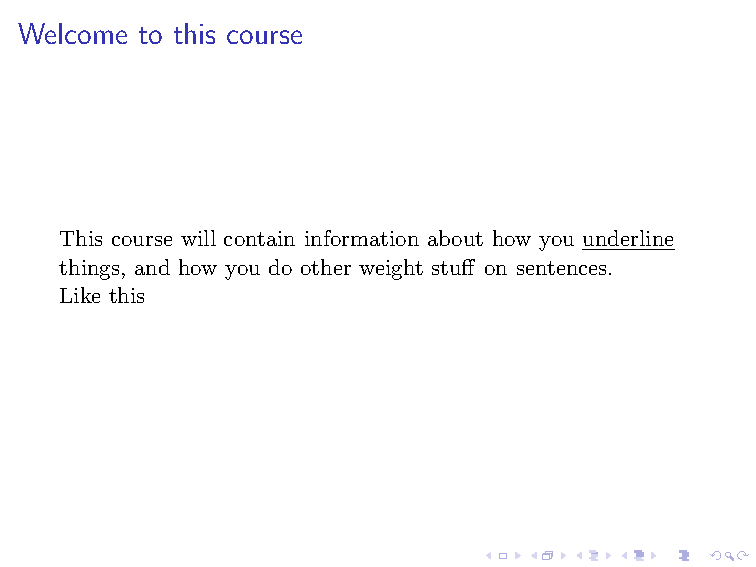
\includegraphics[width=0.8\textwidth]{text/beamer_example.pdf}
	\caption{\LaTeX~Beamer output}
	\label{fig:beamer_example}
\end{figure}%

\end{lstlisting}

The example seen in listing \ref{lst_beamer}, is the Beamer-code for expressing the output. The Beamer-code seen here is only to express output. To make a slideshow using Beamer you have to set up a main document. In this document, all the settings about what theme, colours, inputs (other files), etc., for the slideshow is set up. The editor (TexMaker) only generates a very small amount of the main document, which leaves a lot of setup for the user, if additional settings is wanted. If only a general slideshow is required, the main document will not need much work. A general slideshow is without colours, themes or the need for additional packages.\\
Compared to the Beamer-code the developed language should be made more compact to make slides faster to express.
\\ \\
A test between \LaTeX~Beamer and the developed language will be made to determine which and why one language is better than the other.